\documentclass[a4paper,12pt,english,oneside]{book}

\usepackage{babel}
\usepackage[utf8]{inputenc}
\usepackage[dvipsnames]{xcolor}
\usepackage{hyperref}
\usepackage{tikz}
\usepackage{xspace}
%\usepackage{multirow}
\usepackage{moreverb}
%\usepackage{enumerate}
%\usepackage{enumitem}
%\usepackage{supertabular}
\usepackage{paralist}
%\usepackage{float}
%\usepackage{listings}
\usepackage{scrextend}
\usepackage{pdflscape}
\usepackage{multirow}
\usepackage{booktabs}
\usepackage{fancyvrb}
\usepackage{xstring}

\usepackage{rail}
\railoptions{-h}
\railnontermfont{\rmfamily\itshape}

%\floatstyle{boxed} 
%\restylefloat{figure}

%\usetikzlibrary{arrows,calc}
%\usetikzlibrary{arrows}
\usetikzlibrary{%
  arrows,%
  shapes.misc,% wg. rounded rectangle
  shapes.arrows,%
  chains,%
  matrix,%
  positioning,% wg. " of "
  scopes,%
  decorations.pathmorphing,% /pgf/decoration/random steps | erste Graphik
  shadows%
}

%\renewcommand{\arraystretch}{1.5}

\newcommand{\exeta}{Exeta\xspace}

\newcommand*{\fvn}[1]{\textcolor{Brown}{#1}}
\newcommand*{\fvi}[1]{\textcolor{Magenta}{#1}}
\newcommand*{\fvc}[1]{\textcolor{NavyBlue}{\# #1}}
\newcommand*{\fvhrs}[1]{\href{file:../tutorial/rep/psql/src/#1.sql}{src}}
\newcommand*{\fvhrg}[1]{\href{file:../tutorial/rep/psql/gen/#1.sql}{gen}}
\newcommand*{\fvhre}[1]{\href{file:../tutorial/rep/psql/exe/#1.sql}{exe}}
\newcommand*{\fvhrsSH}[1]{\href{file:../tutorial/rep/bash/src/#1.sh}{src}}
\newcommand*{\fvhrgSH}[1]{\href{file:../tutorial/rep/bash/gen/#1.sh}{gen}}
\newcommand*{\fvhreSH}[1]{\href{file:../tutorial/rep/bash/exe/#1.sh}{exe}}

\title{\exeta}
\author{Martin Proch\'{a}zka}
%\date{2014-05-19}

\begin{document}

\newsavebox{\verbbox}

\maketitle

\tableofcontents

\chapter{Introduction}
%\addcontentsline{toc}{chapter}{Introduction}

\exeta is a framework for processing mutually dependent \emph{tasks} in a distributed heterogeneous computing environment. The framework consists of the following components:
\begin{itemize}
  \item a compiler
  \item a repository
  \item an engine
  \item a console
\end{itemize}
The \emph{compiler} translates task definitions written in \exeta \emph{language} into relational representation which is stored in a \emph{repository}. The repository is utilized by the \emph{engine} that submits tasks to various servers (database, ETL, application, etc.) for execution, then tracks them and updates their \emph{status}. The order of tasks' execution is given by defined \emph{dependencies}. Task processing is monitored and controlled by operations stuff via the operational \emph{console}. % \exeta language enables developers to declare \emph{what}, \emph{where}, and \emph{when} should be executed.

\exeta is designed to minimize both development and operational effort. It is supported by the following features:
\begin{itemize}
  \item code reusability
  \item code generation
  \item tasks grouping
  \item failure recovery
  \item easy deployment
  \item dynamic prioritization
  \item dynamic capacity planning
  %\item reusability of code in different phases of software development (data analysis and implementation)
%\item streamline development by interconnecting data analysis with coding -- data analysis queries can be transformed easily into task scripts 
  %\item operating groups of tasks with or without all their successors or predecessors
%\item comfortable and easy monitoring and operation -- console enables manipulating with groups of tasks, with or without all its predecessors or successors.
\end{itemize}
%\paragraph{\it Development environment}%
%can be used for declaration of components the enterprise computing environment consists of, namely
%\begin{itemize}
%  \item task executors,
%  \item execution schedules, and
%  \item tasks and their mutual dependencies.
%\end{itemize}
%
%\paragraph{\it Templates}%
%are reusable pieces of code used for common generic tasks such as historization in Data Warehousing area.
%
%\paragraph{\it Impact analysis and data lineage tool}%
%\begin{itemize}
%  \item automatic for SQL tasks,
%  \item custom meta-data driven for other types of tasks.
%\end{itemize}
%
%\begin{itemize}
%  \item Server (repository, process, status logging)
%  \item Executors (API)
%  \item Task instances are submitted to executors using \texttt{ssh}/\texttt{scp}.
%\end{itemize}
%
%\section*{What is it?}
%\addcontentsline{toc}{section}{What is it?}
%
%\section*{What is it good for?}
%\addcontentsline{toc}{section}{What is it good for?}
%
%\begin{itemize}
%  \item ELT/ETL (the primary area of application)
%  \item cloud computing
%  \item execution of mutually dependent computations in a distributed heterogeneous computing environment
%\end{itemize}
%
%\section*{Why to choose it?}
%\addcontentsline{toc}{section}{Why to choose it?}
%
%When using standard ETL tools like Informatica, business analysts need to describe their findings collected during data analysis phase in detailed specification that is then handed over to ETL developers. ETL developers transfer this specification into Informatica deliverables (mappings and workflows). Each such handover between different people could lead to  misunderstanding of the specification and therefore cause flaws in the delivery.

%Exeta minimizes such risks as SQL queries created during the data analysis phase can be easily, with almost no change, used as the code of \exeta tasks. This approach decreases costs of development as there is no need to write the same thing in two different ways. It also reduces number of different roles participating in a development team. Both data analysis and code implementation can be done by a single person--the programmer.

%Exeta enables utilization of an  agile software development cycle shown in Figure \ref{fig:0:0:1}.
%
%\begin{figure}
%\begin{enumerate}
%  \item Concept.
%  \item Data analysis.
%  \item Iterative prototyping
%  \begin{enumerate}
%    \item prototype (re)build,
%    \item prototype (re)test,
%    \item requirements refinement.
%  \end{enumerate}
%  \item Deployment into production.
%  \item Production support.
%\end{enumerate}
%\caption{Agile software development cycle.}
%\label{fig:0:0:1}
%\end{figure}
%
%Exeta makes it easy to use reusable pieces of code. These pieces of code can be generated from technical meta-data.

%You need not to buy expensive ETL servers (both HW and SW) and to pay licenses for them. Using \exeta the processing can be done by database servers.

\chapter{Tutorial}

Our tutorial comes from the field of data warehousing and ETL\footnote{Extraction, Transformation, Load} processing in a telecommunication company. Data warehouse stores data from various source systems such as network mediation, billing, CRM\footnote{Customer Relationship Management}, ERP\footnote{Enterprise Resource Planning}, external data sources (e.g., regulators, government, statistical office or marketing agencies) or manually maintained code lists. It keeps detailed data (with limited history), its aggregations (with potentially unlimited history) and data derived from it according to defined business rules. This enables reporting, data analysis, forecasting, customer segmentation, data mining, campaign support, etc. All data processing is performed by the ETL tool. This is in particular the extraction of data from source systems, its loading into the data warehouse, and transformation (consolidation, aggregation, and calculation of derived data).

\section{Architecture}

The data warehouse consists of several layers each serving to a different purpose:
\begin{itemize}
  \item extract layer
  \item stage layer
  \item target layer
\end{itemize}

\subsection{Extract Layer}

The extract layer is placed in the file system of the ETL server. It is a place where extracts from the source systems are delivered to. Extracts are loaded into the stage layer. Extract that is successfully loaded form the extract layer into the stage layer is deleted from the file system by the task that is responsible for loading into the stage layer. It means that the production and the consumption of the extracts are asynchronous.

Extracts form agreed interfaces between source systems and the data warehouse. They must meet strictly defined rules. For example: \begin{list}{}{}\it
\item Each extract is a semicolon separated variable length file.
\item Each string field is delimited by \verb|"|, encoded in unicode, with \verb|\| as an escape character.
\item Each date field is in ISO 8601 format \verb|YYYY-MM-DD|.
\item Each timestamp field is in ISO 8601 format \verb|YYYY-MM-DD HH24:MI:SS|.
\item Each number uses \verb|.| as a decimal point, etc.
\end{list}

In order to minimize volume of data transferred three types of extracts are used:
\begin{itemize}%[(a)]
\item increment,
\item delta,
\item full.
\end{itemize}
\emph{Incremental extracts} are suitable for transactional data that are generated once by the source system and then never changed. An increment needs to be identifiable by a sequence number or by a time stamp. \emph{Delta extracts} are used in cases of frequently modified data. Their first field contains an operation that should by applied to the row to load it into the target table. This operation is \verb|INSERT|, \verb|UPDATE|, or \verb|DELETE|. Each data set populated with delta extracts must have a primary or unique key. \emph{Full extracts} are used for small data sets or for data sets that do not conform to prerequisites on incremental or delta extracts.

\subsection{Stage Layer}

The stage layer is a source for the target layer. It is a database that stores a limited history of extracts. So, it enables reloads of data in the target layer. The stage is not accessible to end users.

\subsection{Target Layer}

\section{Assignment}

%Our first assignment is to
Load a company data provided by the Statistical Office into the data warehouse on regular basis.
% This data can be used for segmentation of customers which can then influence a construction of campaign selection lists, product offerings, etc.
The data consists of two files:
\begin{itemize}
\item \href{file:../tutorial/ext/czso/KLAS80004_CS.20170512000000.dat}{KLAS80004\_CS}
\item \href{file:../tutorial/ext/czso/RES_CS.20170512000000.dat}{RES\_CS}
\end{itemize}
The first one is a code list containing a \emph{classification of economic activities \href{https://en.wikipedia.org/wiki/Statistical_Classification_of_Economic_Activities_in_the_European_Community}{NACE}}, the other contains a company information from the \href{https://www.czso.cz/csu/res/registr_ekonomickych_subjektu}{\emph{Business Register}} (id, name, address, type of ownership, date of establishment and termination, list of NACE activities, and a range of a number of employees). Implement the data processing in the following steps:
\begin{enumerate}
\item Transfer files from an agreed place into the extract layer.
\item Load extracts into the stage layer.
\item Transform data from the stage into the \href{https://en.wikipedia.org/wiki/Third_normal_form}{3NF} in the target layer.
\end{enumerate}
Use \verb|scp| for file transfers. The data warehouse runs on PostgreSQL database server. \exeta runs on a linux host.
%During data analysis the following inputs were identified:
%\begin{itemize}
%\item call data records from the network mediation
%\item invoices from the billing system
%\item customer master data from CRM
%\item surveys from the Statistical Office
%\item manual code list and mapping defining the segmentation
%\end{itemize}
%We assume that the network mediation prepares csv files with call data records (CDR) and places them in a mediation file system. Billing as well as CRM data is not extracted from the production databases, rather it is taken from their standby replicas. (Another option is to use some online replication mechanism like Oracle GoldenGate.) Surveys from the Statistical Office are placed irregularly directly into the extract layer in csv files.

\section{Solution}

\subsection{Database Part}

\subsection{ETL Part}

\subsubsection{\exeta Source}

generic reusable tasks will be developed that 

\begin{table}%
\centering%
\begin{tabular}{r|r|l}%
\toprule%
\multicolumn{2}{r|}{\bf Task classification} & \bf \exeta source file \\
\midrule
\multirow{4}{*}{Generic}
  &     shell & \href{file:../tutorial/rep/100_sh_generic.e}{\tt 100\_sh\_generic.e} \\
  &  database & \href{file:../tutorial/rep/200_db_generic.e}{\tt 200\_db\_generic.e} \\
  &     stage & \href{file:../tutorial/rep/300_edw_stg_generic.e}{\tt 300\_edw\_stg\_generic.e} \\
  &    target & \href{file:../tutorial/rep/400_edw_tgt_generic.e}{\tt 400\_edw\_tgt\_generic.e} \\
\midrule
\multirow{4}{*}{Specific}
  & hierarchy & \href{file:../tutorial/rep/500_main.e}{\tt 500\_main.e} \\
  &   extract & \href{file:../tutorial/rep/600_ext_specific.e}{\tt 600\_ext\_specific.e} \\
  &     stage & \href{file:../tutorial/rep/700_edw_stg_specific.e}{\tt 700\_edw\_stg\_specific.e} \\
  &    target & \href{file:../tutorial/rep/800_edw_tgt_specific.e}{\tt 800\_edw\_tgt\_specific.e} \\
\bottomrule
\end{tabular}
\caption{\exeta source files.}
\end{table}

\subsubsection{Task Code}

\begin{table}%
\centering%
\begin{tabular}{r|r|l}%
\toprule%
\multicolumn{2}{r|}{\bf Task classification} & \bf Task name \\
\midrule
\multirow{6}{*}{Generic}
  & shell
    & \href{file:../tutorial/rep/bash/src/Copy.sh}{\tt Copy} \\
\cmidrule(l){2-3}
  & \multirow{2}{*}{database}
    & \href{file:../tutorial/rep/psql/src/AnalyzeTable.sql}{\tt AnalyzeTable} \\
  & & \href{file:../tutorial/rep/psql/src/DropTable.sql}{\tt DropTable} \\
\cmidrule(l){2-3}
  & \multirow{3}{*}{stage}
    & \href{file:../tutorial/rep/psql/src/LoadStgTable.CreateNew.sql}{\tt LoadStgTable.CreateNew} \\
  & & \href{file:../tutorial/rep/psql/src/LoadStgTable.LoadNew.sql}{\tt LoadStgTable.LoadNew} \\
  & & \href{file:../tutorial/rep/psql/src/LoadStgTable.CopyNew.sql}{\tt LoadStgTable.CopyNew} \\
  & & \href{file:../tutorial/rep/psql/src/LoadStgTable.DropOld.sql}{\tt LoadStgTable.DropOld} \\
\cmidrule(l){2-3}
  & \multirow{7}{*}{target}
    & \href{file:../tutorial/rep/psql/src/LoadTgtTable.CreateNew.sql}{\tt LoadTgtTable.CreateNew} \\
  & & \href{file:../tutorial/rep/psql/src/LoadTgtTable.DropTmp.sql}{\tt LoadTgtTable.DropTmp} \\
  & & \href{file:../tutorial/rep/psql/src/LoadTgtTable.CreateDel.sql}{\tt LoadTgtTable.CreateDel} \\
  & & \href{file:../tutorial/rep/psql/src/LoadTgtTable.CreateIns.sql}{\tt LoadTgtTable.CreateIns} \\
  & & \href{file:../tutorial/rep/psql/src/LoadTgtTable.CreateUpd.sql}{\tt LoadTgtTable.CreateUpd} \\
  & & \href{file:../tutorial/rep/psql/src/LoadTgtTable.LoadDel.sql}{\tt LoadTgtTable.LoadDel} \\
  & & \href{file:../tutorial/rep/psql/src/LoadTgtTable.LoadIns.sql}{\tt LoadTgtTable.LoadIns} \\
\midrule
\multirow{4}{*}{Specific}
  & \multirow{4}{*}{target}
    & \href{file:../tutorial/rep/psql/src/LoadTgtTable.Transform.Activity.sql}{\tt LoadTgtTable.Transform.Activity} \\
  & & \href{file:../tutorial/rep/psql/src/LoadTgtTable.Transform.Party.sql}{\tt LoadTgtTable.Transform.Party} \\
  & & \href{file:../tutorial/rep/psql/src/LoadTgtTable.Transform.PartyActivity.T01.sql}{\tt LoadTgtTable.Transform.PartyActivity.T01} \\
  & & \href{file:../tutorial/rep/psql/src/LoadTgtTable.Transform.PartyActivity.New.sql}{\tt LoadTgtTable.Transform.PartyActivity.New} \\
\bottomrule
\end{tabular}
\caption{Executable tasks.}
\end{table}

\subsubsection{Expanded Instance Tree}

The \exeta source files are translated into relational representation which is stored in the database repository. This representation is expanded into the instance tree. Expansion starts with the task main and proceeds from the top to the bottom. During this process, features are substituted with their values. The expanded instance tree resulting from our source files is shown below. Right to each executable task, the link to its source code, generated code, and executable code is placed marked as \texttt{src}, \texttt{gen}, and \texttt{exe} resp. Calling tasks are mentioned in comments.

\begin{landscape}
\begin{Verbatim}[commandchars=+\[\]]
+fvc[main]
(  +fvc[ProvideExtracts]
   (  +fvc[ProvideExtracts.CzSO]
      (  +fvn[Copy] "+fvi[${EXETA_HOME}/rmt/czso/KLAS80004_CS.csv]"
              "+fvi[${EXETA_HOME}/ext/czso/KLAS80004_CS.${TimeStamp}.dat]" +fvhrsSH[Copy] +fvhreSH[0000000000000001]
      || +fvn[Copy] "+fvi[${EXETA_HOME}/rmt/czso/RES_CS.csv]"
              "+fvi[${EXETA_HOME}/ext/czso/RES_CS.${TimeStamp}.dat]" +fvhrsSH[Copy] +fvhreSH[0000000000000002]
      )
   )
|| +fvc[LoadEDW]
   (  +fvc[LoadStgLayer]
      (  +fvc[LoadStgLayer.CzSO]
         (  +fvc[LoadStgTable czso_klas80004_cs]
            (  +fvc[LoadStgTable.DropNew czso_klas80004_cs]
               (  +fvn[DropTable] +fvi[stg_layer czso_klas80004_cs_20170512000000] +fvhrs[DropTable] +fvhre[0000000000000003]
               )
            -> +fvn[LoadStgTable.CreateNew] +fvi[czso_klas80004_cs] +fvhrs[LoadStgTable.CreateNew] +fvhre[0000000000000004]
            -> +fvn[LoadStgTable.LoadNew] +fvi[czso_klas80004_cs] +fvhrs[LoadStgTable.LoadNew] +fvhrg[0000000000000005] +fvhre[0000000000000005]
            -> +fvn[LoadStgTable.CopyNew] +fvi[czso_klas80004_cs] +fvhrs[LoadStgTable.CopyNew] +fvhrg[0000000000000006] +fvhre[0000000000000006]
               +fvc[when LoadStgTable.LoadNew czso_klas80004_cs skipped]
            -> (  +fvn[LoadStgTable.DropOld] +fvi[czso_klas80004_cs] +fvhrs[LoadStgTable.DropOld] +fvhrg[0000000000000007] +fvhre[0000000000000007]
               || +fvc[LoadStgTable.AnalyzeNew czso_klas80004_cs]
                  (  +fvn[AnalyzeTable] +fvi[stg_layer czso_klas80004_cs_20170512000000] +fvhrs[AnalyzeTable] +fvhre[0000000000000008]
                  )
               )  
            )  
         || +fvc[LoadStgTable czso_res_cs]
            (  +fvc[LoadStgTable.DropNew czso_res_cs]
               (  +fvn[DropTable] +fvi[stg_layer czso_res_cs_20170512000000] +fvhrs[DropTable] +fvhre[0000000000000009]
               )
            -> +fvn[LoadStgTable.CreateNew] +fvi[czso_res_cs] +fvhrs[LoadStgTable.CreateNew] +fvhre[0000000000000010]
            -> +fvn[LoadStgTable.LoadNew] +fvi[czso_res_cs] +fvhrs[LoadStgTable.LoadNew] +fvhrg[0000000000000011] +fvhre[0000000000000011]
            -> +fvn[LoadStgTable.CopyNew] +fvi[czso_res_cs] +fvhrs[LoadStgTable.CopyNew] +fvhrg[0000000000000012] +fvhre[0000000000000012]
               +fvc[when LoadStgTable.LoadNew czso_res_cs skipped]
            -> (  +fvn[LoadStgTable.DropOld] +fvi[czso_res_cs] +fvhrs[LoadStgTable.DropOld] +fvhrg[0000000000000013] +fvhre[0000000000000013]
               || +fvc[LoadStgTable.AnalyzeNew czso_res_cs]
                  (  +fvn[AnalyzeTable] +fvi[stg_layer czso_res_cs_20170512000000] +fvhrs[AnalyzeTable] +fvhre[0000000000000014]
                  )
               )  
            )  
         )  
      )  
   || +fvc[LoadTgtLayer]
      (  +fvc[LoadTgtTable activity]
         +fvc[when LoadStgTable czso_klas80004_cs succeeded]
         (  
            (  (  +fvc[LoadTgtTable.DropNew activity]
                  (  +fvn[DropTable] +fvi[wrk_area activity_n] +fvhrs[DropTable] +fvhre[0000000000000015]
                  )
               -> +fvn[LoadTgtTable.CreateNew] +fvi[activity] +fvhrs[LoadTgtTable.CreateNew] +fvhre[0000000000000016]
               )  
            || +fvn[LoadTgtTable.DropTmp] +fvi[activity] +fvhrs[LoadTgtTable.DropTmp] +fvhrg[0000000000000017] +fvhre[0000000000000017]
            )  
         -> +fvn[LoadTgtTable.Transform.Activity] +fvhrs[LoadTgtTable.Transform.Activity] +fvhre[0000000000000018]
         -> (  (  +fvc[LoadTgtTable.DropIns activity]
                  (  +fvn[DropTable] +fvi[wrk_area activity_i] +fvhrs[DropTable] +fvhre[0000000000000019]
                  )
               -> +fvn[LoadTgtTable.CreateIns] +fvi[activity] +fvhrs[LoadTgtTable.CreateIns] +fvhre[0000000000000020]
               )  
            || (  +fvc[LoadTgtTable.DropUpd activity]
                  (  +fvn[DropTable] +fvi[wrk_area activity_u] +fvhrs[DropTable] +fvhre[0000000000000021]
                  )
               -> +fvn[LoadTgtTable.CreateUpd] +fvi[activity] +fvhrs[LoadTgtTable.CreateUpd] +fvhrg[0000000000000022] +fvhre[0000000000000022]
               )  
            || (  +fvc[LoadTgtTable.DropDel activity]
                  (  +fvn[DropTable] +fvi[wrk_area activity_d] +fvhrs[DropTable] +fvhre[0000000000000023]
                  )
               -> +fvn[LoadTgtTable.CreateDel] +fvi[activity] +fvhrs[LoadTgtTable.CreateDel] +fvhre[0000000000000024]
               ) 
            )  
         -> +fvn[LoadTgtTable.LoadIns] +fvi[activity] +fvhrs[LoadTgtTable.LoadIns] +fvhre[0000000000000025]
         -> +fvn[LoadTgtTable.LoadDel] +fvi[activity] +fvhrs[LoadTgtTable.LoadDel] +fvhre[0000000000000026]
         )  
      || +fvc[LoadTgtTable party]
         +fvc[when LoadStgTable czso_res_cs succeeded]
         (  
            (  (  +fvc[LoadTgtTable.DropNew party]
                  (  +fvn[DropTable] +fvi[wrk_area party_n] +fvhrs[DropTable] +fvhre[0000000000000027]
                  )
               -> +fvn[LoadTgtTable.CreateNew] +fvi[party] +fvhrs[LoadTgtTable.CreateNew] +fvhre[0000000000000028]
               )  
            || +fvn[LoadTgtTable.DropTmp] +fvi[party] +fvhrs[LoadTgtTable.DropTmp] +fvhrg[0000000000000029] +fvhre[0000000000000029]
            )  
         -> +fvn[LoadTgtTable.Transform.Party] +fvhrs[LoadTgtTable.Transform.Party] +fvhre[0000000000000030]
         -> (  (  +fvc[LoadTgtTable.DropIns party]
                  (  +fvn[DropTable] +fvi[wrk_area party_i] +fvhrs[DropTable] +fvhre[0000000000000031]
                  )
               -> +fvn[LoadTgtTable.CreateIns] +fvi[party] +fvhrs[LoadTgtTable.CreateIns] +fvhre[0000000000000032]
               )  
            || (  +fvc[LoadTgtTable.DropUpd party]
                  (  +fvn[DropTable] +fvi[wrk_area party_u] +fvhrs[DropTable] +fvhre[0000000000000033]
                  )
               -> +fvn[LoadTgtTable.CreateUpd] +fvi[party] +fvhrs[LoadTgtTable.CreateUpd] +fvhrg[0000000000000034] +fvhre[0000000000000034]
               )  
            || (  +fvc[LoadTgtTable.DropDel party]
                  (  +fvn[DropTable] +fvi[wrk_area party_d] +fvhrs[DropTable] +fvhre[0000000000000035]
                  )
               -> +fvn[LoadTgtTable.CreateDel] +fvi[party] +fvhrs[LoadTgtTable.CreateDel] +fvhre[0000000000000036]
               )  
            )  
         -> +fvn[LoadTgtTable.LoadIns] +fvi[party] +fvhrs[LoadTgtTable.LoadIns] +fvhre[0000000000000037]
         -> +fvn[LoadTgtTable.LoadDel] +fvi[party] +fvhrs[LoadTgtTable.LoadDel] +fvhre[0000000000000038]
         )  
      || +fvc[LoadTgtTable party_activity]
         +fvc[when LoadTgtTable party succeeded]
         +fvc[  &  LoadTgtTable activity succeeded]
         (  
            (  (  +fvc[LoadTgtTable.DropNew party]
                  (  +fvn[DropTable] +fvi[wrk_area party_activity_n] +fvhrs[DropTable] +fvhre[0000000000000039]
                  )
               -> +fvn[LoadTgtTable.CreateNew] +fvi[party_activity] +fvhrs[LoadTgtTable.CreateNew] +fvhre[0000000000000040]
               )  
            || +fvn[LoadTgtTable.DropTmp] +fvi[party_activity] +fvhrs[LoadTgtTable.DropTmp] +fvhrg[0000000000000041] +fvhre[0000000000000041]
            )  
         -> +fvc[LoadTgtTable.Transform.party_activity]
            (  
               (  +fvn[LoadTgtTable.Transform.PartyActivity.T01] +fvhrs[LoadTgtTable.Transform.PartyActivity.T01] +fvhre[0000000000000042]
               -> +fvn[LoadTgtTable.Transform.PartyActivity] +fvhrs[LoadTgtTable.Transform.PartyActivity] +fvhre[0000000000000043]
               )  
            )  
         -> (  (  +fvc[LoadTgtTable.DropIns party]
                  (  +fvn[DropTable] +fvi[wrk_area party_activity_i] +fvhrs[DropTable] +fvhre[0000000000000044]
                  )
               -> +fvn[LoadTgtTable.CreateIns] +fvi[party_activity] +fvhrs[LoadTgtTable.CreateIns] +fvhre[0000000000000045]
               )  
            || (  +fvc[LoadTgtTable.DropUpd party]
                  (  +fvn[DropTable] +fvi[wrk_area party_activity_u] +fvhrs[DropTable] +fvhre[0000000000000046]
                  )
               -> +fvn[LoadTgtTable.CreateUpd] +fvi[party_activity] +fvhrs[LoadTgtTable.CreateUpd] +fvhrg[0000000000000047] +fvhre[0000000000000047]
               )  
            || (  +fvc[LoadTgtTable.DropDel party]
                  (  +fvn[DropTable] +fvi[wrk_area party_activity_d] +fvhrs[DropTable] +fvhre[0000000000000048]
                  )
               -> +fvn[LoadTgtTable.CreateDel] +fvi[party_activity] +fvhrs[LoadTgtTable.CreateDel] +fvhre[0000000000000049]
               )  
            )  
         -> +fvn[LoadTgtTable.LoadIns] +fvi[party_activity] +fvhrs[LoadTgtTable.LoadIns] +fvhre[0000000000000050]
         -> +fvn[LoadTgtTable.LoadDel] +fvi[party_activity] +fvhrs[LoadTgtTable.LoadDel] +fvhre[0000000000000051]
         )  
      )  
   )  
)  
\end{Verbatim}
\end{landscape}

\chapter{Concepts}

In this chapter, basic \exeta concepts are presented. The \exeta language is introduced -- how to define tasks in \exeta language. Compilation -- translation of task definitions to task instances forming an instance tree is shown. A processing of task instances (so called task instance runs) is explained with an emphases on statuses they can get into.

\section{Definition}

The main \exeta asset is a \emph{task}. Each task has its header consisting of a \emph{name} and a set of \emph{identifiers}, a set of \emph{features}, a \emph{body}, and \emph{rules}. Tasks can be called from other tasks with identifiers' and features' values assigned.

Both identifiers and features are used to transfer an information from outside of a task call into its inside and to parametrize a code executed by the task. They differ in one important aspect: The task name together with its identifier values uniquely identifies a task instance. There cannot be more task instances of the same name and the same identifier values in \exeta. The importance of identifiers in the identification of task instances is discussed in more detail further on.

%\subsubsection{Body}
The task body determines what the task actually does. There are following three possibilities:
\begin{itemize}
\item The task calls other tasks.
\item The task executes its code.
\item The task generates a code first and then executes the generated code.
\end{itemize}
%The third possibility has two variants: either the code is generated each time the task is called, or the code is generated just by the very first call of the task.
A server that generates a code is called \emph{generator} and it is set by a system feature \verb|generator|.
A server that executes a code is called \emph{executor} and it is set by a system feature \verb|executor|.

If the code of a generating task contains not escaped \verb+${TimeStamp}+ (the only dynamic feature that contains a value that is known at run-time, not any sooner) then the task is generated each time just before it is executed. Otherwise, it is generated just once at the time of deployment.

To declare which tasks should be executed in the computing environment there is one special task called \verb|main|. This is the task all other tasks that should be executed are called from, either directly or transitively.

A task \verb|LoadTable| that loads data into a Data Warehouse table is defined in the following way:
\begin{verbatim}
task LoadTable Schema Table
  call PrepareWorkArea.${Method} ${Schema} ${Table}
    -> LoadWorkTable.${Schema}.${Table}
    -> LoadTargetTable.${Method} ${Schema} ${Table}
;
\end{verbatim}

%\subsubsection{Parameters}
It has two identifiers \verb|Schema| and \verb|Table| that unique\-ly identify what table is loaded, and two parameters \verb|IdList| and \verb|Method| that specify how the table is loaded.
%\subsubsection{Features}
Further, there is a \emph{with} clause that lists task features. In our case, there is just one feature \verb|recovery|--a system feature defining \exeta behavior in case of task's failure (for details, see Subsection \ref{subsec:rec-fea}).

The first kind of task's body is demonstrated by the task \verb|LoadTable| mentioned above. This task \emph{calls in sequence} following three other tasks:
\begin{itemize}
\item \verb|PrepareWorkArea.${Method}|,
\item \verb|LoadWorkTable.${Schema}.${Table}|, and
\item \verb|LoadTargetTable.${Method}|
\end{itemize}
with identifier and parameter values passed to them. Values of both of them are denoted using Unix shell notation, i.e., the value of an identifier \verb|table| is denoted by \verb|${table}|. Calls of all tasks in this example demonstrate another powerful \exeta feature--called task names can contain variable values. It enables \emph{polymorphism} introduced by object-oriented programming languages. In our case, there is one generic task for a load of any table. What code is actually executed depends on specific values of identifiers or parameters \verb|Schema|, \verb|Table|, and  \verb|Method|. A different code is executed for a different method (such as \verb|SCD1|, \verb|SCD2|, \verb|Increment|, etc.) and different tables in different schemata. See the following code for examples of \verb|LoadTable| task calls:
%\begin{verbatim}
%task LoadStageDaily
%  calls in parallel (
%    LoadTable ( "STG_DB" "S_ORG_EXT" ) {
%      with
%        IdList "ROW_ID"
%        Method "Delta"
%      when
%        CheckSource ( "CRM" "S_ORG_EXT" ) succeeded
%      }
%    LoadTable ( "STG_DB" "S_ASSET" ) {
%      with
%        IdList "ROW_ID"
%        Method "Delta"
%      when
%        CheckSource ( "CRM" "S_ASSET" ) succeeded
%      }
%    )
%;
%\end{verbatim}
\begin{verbatim}
task LoadTargetDaily
with executor = mypsql
  ,  schedule = " 0 0 * * * "
call LoadTable DW_DB DW_ACCOUNT
     with IdList = ( ACCOUNT_ID )
       ,  Method = SCD2
     when LoadTable STG_DB S_ORG_EXT succeeded
  || LoadTable DW_DB DW_SUBSCRIBER
     with IdList = ( SUBSCRIBER_ID )
       ,  Method = SCD2
     when LoadTable DW_DB  DW_ACCOUNT succeeded
       &  LoadTable STG_DB S_ASSET    succeeded
;
\end{verbatim}
Identifiers, parameters, and features are inherited from task's ancestors and they can be re-assigned by children.

%\subsection{Task Dependencies}

%Task call--task name, parameters, or features can contain variables.\\
%Task instance--all variables are substituted, including \verb|timestamp|.

A task name together with identifiers and an executor the task is assigned to uniquely identifies the task instance as well as task script and its location in the \exeta file system repository.

\emph{When condition} and time related system features:
\begin{verbatim}
task LoadTargetMonthly
with schedule = " 0 0 * * 0 "
call LoadTable DW_DB DW_SEGMENTATION
;
task LoadTargetDaily
with schedule = " 0 0 * * * "
call LoadTable DW_DB DW_CAMPAIGN
     when LoadTable DW_DB DW_SEGMENTATION succeeded
;
\end{verbatim}

The check if the load of the table \verb|DW_CAMPAIGN|
%\begin{center}
%\verb|LoadTable( "DW_DB" "DW_CAMPAIGN_SELECTION_LIST" )|
%\end{center}
can be started with a time stamp given by a schedule \verb|Daily| is done in following steps:
\begin{enumerate}
\item Get a maximum time stamp from the schedule \verb|Monthly| assigned to the task call
\verb|LoadTable| \verb|DW_DB| \verb|DW_SEGMENTATION|
that is less or equal to the current time stamp of the task call
\verb|LoadTable| \verb|DW_DB| \verb|DW_CAMPAIGN|.
\item If the task call
\verb|LoadTable| \verb|DW_DB| \verb|DW_SEGMENTATION|
finished with the required status for this time stamp (i.e., succeeded in our example) then start the task call
\verb|LoadTable| \verb|DW_DB| \verb|DW_CAMPAIGN|,
otherwise postpone it.
\end{enumerate}

%\subsection{Main Task}
In our example, \verb|main| could look like this:
\begin{verbatim}
task main
call LoadDW
;
task LoadDW
with executor = mypsql
submit same after 5 m 5 times then suspend when failed
submit next when succeeded
submit next when skipped
call LoadDWStg
  || LoadDWTgtDaily
  || LoadDWTgtMonthly
;
\end{verbatim}

%This guaranties that following two subtasks (and their subtasks, recursively down to executable tasks) will be executed in computational environment:
%\begin{itemize}
%  \item \verb|CheckSource|
%  \item \verb|LoadDataWarehouse|
%\end{itemize}

%\begin{flushleft}
%\begin{tabular}{@{}p{.05\textwidth}@{}p{.95\textwidth}@{}}
%& \begin{verbatim}
%task CheckSource
%  calls in parallel (
%    CheckSourceDaily
%    CheckSourceWeekly
%    CheckSourceMonthly
%  )
%;
%\end{verbatim}
%\end{tabular}
%\end{flushleft}
%
%\begin{flushleft}
%\begin{tabular}{@{}p{.05\textwidth}@{}p{.95\textwidth}@{}}
%& \begin{verbatim}
%task CheckSourceDaily
%  with
%    schedule "DailyAt0314"
%  calls in parallel (
%    CheckSource ( "CRM" "S_ORG_EXT" )
%    CheckSource ( "CRM" "S_ASSET" )
%  )
%;
%\end{verbatim}
%\end{tabular}
%\end{flushleft}
%
%\begin{flushleft}
%\begin{tabular}{@{}p{.05\textwidth}@{}p{.95\textwidth}@{}}
%& \begin{verbatim}
%task CheckSource ( System Object )
%  with
%    executor "${System}"
%  executes code
%;
%\end{verbatim}
%\end{tabular}
%\end{flushleft}
%
%\begin{flushleft}
%\begin{tabular}{@{}p{.05\textwidth}@{}p{.95\textwidth}@{}}
%& \begin{verbatim}
%task LoadDW
%  with
%    executor "DataWarehouse"
%  calls in parallel (
%    LoadDWDaily
%    LoadDWWeekly
%    LoadDWMonthly
%  )
%;
%\end{verbatim}
%\end{tabular}
%\end{flushleft}
%
%\begin{flushleft}
%\begin{tabular}{@{}p{.05\textwidth}@{}p{.95\textwidth}@{}}
%& \begin{verbatim}
%task LoadDWDaily
%  with
%    schedule "Daily"
%  calls in parallel (
%    LoadStageDaily
%    LoadTargetDaily
%  )
%;
%\end{verbatim}
%\end{tabular}
%\end{flushleft}

%\subsection{Task Parameters}

\subsection{Features}\label{sec:fea}

\subsubsection{Custom}

\subsubsection{System}

There are several features--so called \emph{system features}--that have a special meaning in \exeta and influence the way tasks are executed. System features are the following:
\begin{itemize}
\item \verb|executor|
\item \verb|generator|
\item \verb|timestamp|
\item \verb|schedule|
%\item \verb|importance|
%\item \verb|consumption|
\end{itemize}
Some of them have been already mentioned in the text above. Here, their complete list with a brief explanation of each of them is provided. When not defined explicitly a feature is set to its default value. Default values are underlined.

Any system feature can be set for a task instance by its parental instance or it can be passed into a task instance as a parameter.

\exeta recognizes two different types of executing servers defined by the following two system features:
\begin{itemize}
\item \verb|executor|
\item \verb|generator|
\end{itemize}

The feature \verb|executor| determines a server or application that \emph{executes} the task code.

The feature \verb|generator| specifies a server or application that \emph{generates} (and possibly installs) a code to be executed. It is used by tasks that execute a generated code. Such tasks are executed in two steps:%
\begin{inparaenum}[(i)]
\item first, the task code is executed by the generator; then
\item the output from the first step is executed by the task executor.
\end{inparaenum}

\subsubsection{Run-time}

TOTO BUDE NASTAVITELNÉ AŽ V RUN-TIME REPOSITORY. IMPORTANCE A CAPACITY SE TOTIŽ VÁŽE NA TASK INSTANCE.

Usually, there is more candidates to run on the same executor at the same time, but not all of them can be executed at once as resources of each executor are limited. Selection which candidate will be passed to its executor is controlled by two features
\begin{itemize}
    \item capacity, and
    \item importance.
\end{itemize}
Task instance's capacity tells us how many per cents of executor's resources are consumed by the task instance.

Which task instances should be passed to a given executor with a capacity $C_E$ for execution?
\begin{enumerate}
    \item Let $C_R$ be a sum of capacities of all task instances running on this executor.
    \item If there is a submitted task instance with this executor and a capacity $C$ such that
    $C\le C_E-C_R$, then run this instance on the executor.
    \item Repeat previous steps until no task instance is selected.
\end{enumerate}

\subsection{Body}

\subsubsection{Execute}

Until now, all tasks called other tasks within their bodies. No task executed any piece of executable code directly. Now, we will show how to link an \exeta task to a code to be executed.

Let us see the following task:
\begin{verbatim}
task LoadTable.DW_DB.DW_ACCOUNT execute ;
\end{verbatim}
There is just a note in the task's body that it executes some code, but the code is missing there. Instead of including the code in \exeta definition file the code is placed in separate file the path and name of which is fully determined by task's \emph{executor} and \emph{name}. In our case, as \verb|executor=mypsql| and \verb|mypsql| file exists in \verb|${EXETA_HOME}/rep/psql/srv| folder, it is
\begin{verbatim}
${EXETA_HOME}/rep/psql/src/LoadTable.DW_DB.DW_ACCOUNT
\end{verbatim}
where usually \verb|EXETA_HOME=/opt/exeta|.
Separating \exeta definition file from executable codes makes a development easier as the executable code can be developed using development tools specific for a given executor.

\subsubsection{Generate an Execute}

\subsubsection{Call}

\subsection{Rules}

\subsubsection{Recovery}\label{subsec:rec-fea}

Recovery of failed task instances is controlled by a \emph{recovery rule}. It determines what happens after task's failure. A time between task's failure and its recovery attempt is controlled by the next item \emph{wait}. Recovery rule has the follewing syntax
\begin{flushleft}
\begin{tabular}{l}
\verb|when failed|\\
$\{$ \verb|then|\\
\textcolor{white}{$\{$} $[$ \verb|wait| $\langle Number\rangle$ ( \verb|s| $\mid$ \verb|m| $\mid$ \verb|h| ) \verb|and| $]$\\
\textcolor{white}{$\{$} ( \verb|fail caller| $\mid$ \verb|submit same| )\\
\textcolor{white}{$\{$} ( \verb|once| $\mid$ \verb|twice| $\mid$ $\langle\textit{Number3+}\rangle$ \verb|times| )\\
$\}$\\
\textcolor{white}{$\{$} \verb|then| ( \verb|succeed| $\mid$ \verb|skip| $\mid$ \verb|suspend| $\mid$ \verb|fail caller| $\mid$ \verb|submit same| )
\end{tabular}
\end{flushleft}
where \emph{Number} is a natural number;
\emph{Action} takes one of the following values:
\begin{labeling}[ --]{\texttt{fail caller}}
\item [\texttt{succeed}] leaves the failed task in the status \verb|succeeded|,% after all recovery attempts have been exhausted,
%
\item [\texttt{skip}] leaves the failed task in the status \verb|skipped|,% after all recovery attempts have been already exhausted,
%
\item [\texttt{suspend}] leaves the failed task in the status \verb|suspended| %after all recovery attempts have been already exhausted
and waits for manual resolution of the problem,
%
\item [\texttt{fail caller}] raises the failure to a calling task,
%
\item [\texttt{submit same}] re-submits (restarts) the failed task;
\end{labeling}
%Both these run-time parameters are set to its default values during the first deployment of the task onto production and controlled by an operational support without a need of recompilation and redeployment.

\subsubsection{Submission}

Schedule features together determine%
\begin{inparaenum}[(i)]
    \item which time stamps are passed to a task instance, and
    \item when a task instance is started.
\end{inparaenum}
It is controlled by the following two features:
\begin{itemize}
    \item \verb|schedule|
    \item \verb|timestamp|
\end{itemize}
The feature \verb|schedule| is a list of one of the following forms:
\begin{center}
    \verb|( submit same when succeeded )|
\end{center}
or
\begin{center}
    \verb|( submit same when skipped )|
\end{center}
or
\begin{center}
    \verb|( submit next by| \emph{plan} \verb|after| \emph{base} \verb|)|
\end{center}
or
\begin{center}
    \verb|( when| \emph{final-status} \verb|then submit next by| \emph{plan} \verb|after| \emph{base} \verb|)|
\end{center}
or
\begin{center}
    \begin{tabular}{l}
        \verb|( submit next by| \emph{plan} \verb|after| \emph{base} \verb|when| \emph{final-status-1}\\
        \verb|( submit next by| \emph{plan} \verb|after| \emph{base} \verb|when| \emph{final-status-2}
    \end{tabular}
\end{center}
consisting of the following objects: the \emph{final-status} -- specifies the final status (\verb|succeeded| or \verb|skipped|); the \emph{base} -- determines the base the next value of time stamp is derived from; the \emph{plan} -- specifies the sequence of time stamps passed to the task and all its children as a value of the feature \verb|timestamp|. It uses extended \verb|cron| notation as you can see in the following example:
\begin{verbatim}
schedule = ( "14 3 1 * *" "0 0 2 * *" )
\end{verbatim}
This schedule generates following sequence of time stamps:
\begin{flushleft}
    \begin{tabular}{c}
        \vdots \\
        \texttt{2015-05-01 03:14} \\
        \texttt{2015-05-02 00:00} \\
        \texttt{2015-06-01 03:14} \\
        \texttt{2015-06-02 00:00} \\
        \vdots
    \end{tabular}
\end{flushleft}
There are two ways how to determine the next value of this system feature \verb|timestamp| that is passed to a given task instance:
%. The \emph{base} value the next time stamp in the schedule sequence is taken from makes the difference. It is either the last used value of \verb|timestamp| feature the task instance have already run with or the time when the last task instance has finished:
\begin{itemize} %[ --]{\underbar{\texttt{submit future}}}
    \item \underbar{\texttt{submit next}}
    
    A new task instance will be submitted with a time stamp given by its schedule that immediately follows the time stamp of the \emph{last} (just finished) task call;
    \item \texttt{submit future}
    
    A new task call will be submitted with a time stamp given by its schedule that immediately follows the current (real) time.
\end{itemize}
The features \verb|schedule| can be set in the task declaration only (not in the task call) and once defined it cannot be redefined in successor tasks. %This way the \emph{unity of time} is guarantied.
The feature \verb|timestamp| is set internally by \exeta system; it can be set in no \exeta feature declaration.
%
%\subsubsection{Execution related features}
%
%The order of task instances execution is influenced by the following two features:
%\begin{itemize}
%\item\verb|importance|,
%\item\verb|capacity|.
%\end{itemize}
%The higher the importance of the task instance is the sooner it is executed (assuming all its start conditions are fulfilled).
%
%The task instance capacity says how much of the task executor's capacity it consumes. In an extreme case, the task instance capacity equals its executor's capacity which means that the task instance runs on the executor alone.

\subsection{Code}

\verb!${EXETA_HOME}!\\
\verb!+-bin!\\
\verb!+-doc!\\
\verb!+-rep!\\
\verb!  +-!$\langle\textit{server type name}\rangle$\\
\verb!    +-bin!\\
\verb!    | +-fail!\\
\verb!    | +-generate!\\
\verb!    | +-run!\\
\verb!    | +-status!\\
\verb!    +-src!\\
\verb!    | +-!$\langle\textit{task name 1}\rangle$\\
\verb!    | +-!$\langle\textit{task name 2}\rangle$\\
\verb!    | | !$\cdots$\\
\verb!    | +-!$\langle\textit{task name i}\rangle$\\
\verb!    +-srv!\\
\verb!    | +-!$\langle\textit{server name 1}\rangle$\\
\verb!    | +-!$\langle\textit{server name 2}\rangle$\\
\verb!    | | !$\cdots$\\
\verb!    | +-!$\langle\textit{server name j}\rangle$\\
\verb!    +-wrk!\\
\verb!      +-!$\langle\textit{task name 1}\rangle$\verb!.f!\\
\verb!      +-!$\langle\textit{task name 1}\rangle$\verb!.g!\\
\verb!      +-!$\langle\textit{task name 1}\rangle$\verb!.s!\\
\verb!      +-!$\langle\textit{task name 2}\rangle$\verb!.f!\\
\verb!      +-!$\langle\textit{task name 2}\rangle$\verb!.g!\\
\verb!      +-!$\langle\textit{task name 2}\rangle$\verb!.s!\\
\verb!      | !$\cdots$\\
\verb!      +-!$\langle\textit{task name k}\rangle$\verb!.f!\\
\verb!      +-!$\langle\textit{task name k}\rangle$\verb!.g!\\
\verb!      +-!$\langle\textit{task name k}\rangle$\verb!.s!\\

\section{Compilation}

\section{Processing}

\subsection{Statuses}

Processing of any \emph{task instance} begins when it is \emph{submitted} with all its parameters and features substituted with values. The task instance can be submitted either%
\begin{inparaenum}[(i)]
\item manually by operational support (typically the new task instance), or
\item automatically when the previous instance of the same task has just finished successfully.
\end{inparaenum}

The submitted instance of the task does not start immediately. More accurately, it is ready to run and it is actually started when all task instances it depends on get into required statuses as specified by its start condition. At this moment the status of the task instance is changed to \emph{running} and its code is passed to the executor for execution.

If the processing is finished successfully without any error the status is set to \verb|succeeded| and the next run of this task instance is scheduled and submitted. Otherwise, the status is changed to \verb|failed|.

The failed task instance can be \emph{recovered}. It depends on a selected recovery method and a number of recovery attempts. The recovery means that the task instance status is changed back to \verb|submitted|. However, if a number of retries has been already exhausted the task instance is switched into the status \verb|suspended|.

A task instance in any of statuses except the \verb|running| status can be \emph{blocked}. Once blocked the instance can be \emph{unblocked}.

If the task instance need to succeed the number of its recovery attempts must be set to \verb|unlimited|.

\begin{figure}
\centering
\bigskip
\bigskip
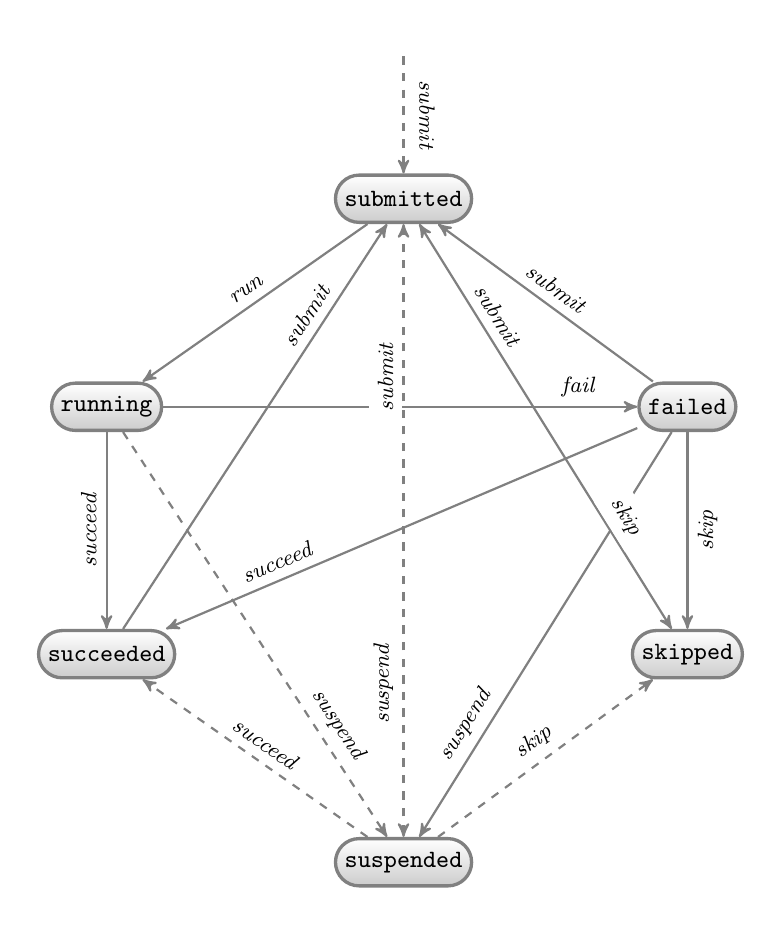
\begin{tikzpicture}
    [   >=stealth'
    ,   thick
    ,   black!50
    ,   text=black
    %,   every new ->/.style={shorten >=1pt}    %,   shorten >=1pt
    ,   status/.style=
            {   % The shape:
                rectangle
            ,   minimum size=6mm
            ,   rounded corners=3mm
            ,   % The rest
                very thick
            ,   draw=black!50
            ,   top color=white
            ,   bottom color=black!20
            ,   font=\ttfamily\small\bfseries %\sffamily\scriptsize\bfseries
            }
    %,   graphs/every graph/.style={edges=rounded corners}
    ]

    \matrix[column sep=20mm, row sep=20mm] {
                                      & \node(H){};                  &                            \\[-5mm]
                                      & \node[status](N){submitted}; &                            \\
         \node[status](R){running};   &                              & \node[status](F){failed};  \\[5mm]
         \node[status](S){succeeded}; &                              & \node[status](P){skipped}; \\
                                      & \node[status](C){suspended};  &                            \\
    };
    \draw[->,dashed](H)--(N) node[sloped,midway,above=2pt]{\it\footnotesize submit};
    \draw[->](N)--(R) node[sloped,midway,above]{\it\footnotesize run};
    \draw[<-](S)--(R) node[sloped,midway,above]{\it\footnotesize succeed};
    \draw[<-](P)--(F) node[sloped,midway,below]{\it\footnotesize skip};
    \draw[->](R)--(F) node[sloped,very near end,above,fill=white]{\it\footnotesize fail};
    \draw[->](F)--(N) node[sloped,midway,above]{\it\footnotesize submit};
    \draw[->](F)--(S) node[sloped,near end,above]{\it\footnotesize succeed};
    \draw[->](F)--(C) node[sloped,near end,above]{\it\footnotesize suspend};
    \draw[->,dashed](C)--(S) node[sloped,midway,above]{\it\footnotesize succeed};
    \draw[->,dashed](C)--(P) node[sloped,midway,above]{\it\footnotesize skip};
    \draw[->,dashed](R)--(C) node[sloped,near end,above]{\it\footnotesize suspend};
    \draw[->](S)--(N) node[sloped,near end,above]{\it\footnotesize submit};
    \draw[<->](N)--(P)
        node[sloped,near start,above]{\it\footnotesize submit}
        node[sloped,near end,above,fill=white]{\it\footnotesize skip};
    \draw[<->,dashed](C)--(N)
    node[sloped,near end,above,fill=white]{\it\footnotesize submit}
    node[sloped,near start,above]{\it\footnotesize suspend};
        \end{tikzpicture}
\bigskip
\bigskip
\caption{Run status transition diagram.}
\label{fig:3:1}
\end{figure}

\subsection{Caller Status Evaluation}

%It is sufficient to define how to derive a status of \verb+A || B+ from statuses of \verb+A+ and \verb+B+ as % The construct
%\[\texttt{A -> B}\quad\equiv\quad\texttt{A || ( B when A succeeded | A skipped )}\]
%Operator \verb+->+ (in sequence) applied onto more than two arguments can be substituted with repeated application of operator \verb+||+ (in parallel) each on just two arguments, as
%\[\texttt{A || B || }\ldots\texttt{ || C}\quad\equiv\quad\texttt{A || ( B || }\ldots\texttt{ || C )}\]

ATTENTION: If
\begin{displaymath}
\texttt{A}_1\quad\texttt{->}\quad\texttt{A}_2\quad\texttt{->}\quad\ldots\quad\texttt{->}\quad\texttt{A}_n,
\end{displaymath}
then $\texttt{A}_i$ cannot run with the next value of \verb|TimeStamp| before $\texttt{A}_n$ has succeeded or skipped for any $i\in\{1,\ldots,n\}$. Otherwise, an object created by $\texttt{A}_i$ and used by some $\texttt{A}_j$, $i<j$, would be recreated by a new run of $\texttt{A}_i$.

\begin{landscape}
%\ctable
%[caption=Status of \texttt{in sequence(A)} and \texttt{in parallel(A)}.]
%{c}
%{}
%{
%\FL
%$\textrm{status of }\texttt{in sequence(A)} = \textrm{status of }\texttt{in parallel(A)} = \textrm{status of }\texttt{A}$
%\LL
%}
%%
\begin{table}
	\centering
	%\tnote{There is no run of the instance \texttt{A} with a given value of \texttt{timestamp}.}
	%\tnote[b]{There is no run of the instance \texttt{B} with a given value of \texttt{timestamp}.}
	\begin{tabular}{c|c|ccccccc}
		\toprule
		\multicolumn{2}{c|}{\multirow{2}{*}{\tt A || B}} & \multicolumn{7}{c}{\tt B} \\
		\cmidrule(rl){3-9}
		\multicolumn{2}{c|}{} & \tt submitted & \tt running & \tt failed   & \tt suspended & \tt succeeded  & \tt skipped & \rm -- \\
		\midrule
		\multirow{6}{*}{\tt A}
		& \tt submitted & \tt submitted & \tt running & \tt running & \tt running   & \tt running   & \tt running   & \tt submitted \\
		& \tt running   & \tt running   & \tt running & \tt running & \tt running   & \tt running   & \tt running   & \tt running   \\
		& \tt failed    & \tt running   & \tt running & \tt failed  & \tt failed    & \tt failed    & \tt failed    & \tt failed    \\
		& \tt suspended & \tt running   & \tt running & \tt failed  & \tt suspended & \tt suspended & \tt suspended & \tt suspended \\
		& \tt succeeded & \tt running   & \tt running & \tt failed  & \tt suspended & \tt succeeded & \tt succeeded & \tt succeeded \\
		& \tt skipped   & \tt running   & \tt running & \tt failed  & \tt suspended & \tt succeeded & \tt skipped   & \tt skipped   \\
		& \rm --        & \tt submitted & \tt running & \tt failed  & \tt suspended & \tt succeeded & \tt skipped   & \rm --        \\
		\bottomrule
	\end{tabular}
	\caption{Status of \texttt{A || B}.}
\end{table}
\begin{table}
	\centering
	%\tnote{There is no run of the instance \texttt{A} with a given value of \texttt{timestamp}.}
	%\tnote[b]{There is no run of the instance \texttt{B} with a given value of \texttt{timestamp}.}
	\begin{tabular}{c|c|cccccc}
		\toprule
		\multicolumn{2}{c|}{\multirow{2}{*}{\tt A -> B}} & \multicolumn{5}{c}{\tt B} \\
		\cmidrule(rl){3-8}
		\multicolumn{2}{c|}{} & \tt submitted & \tt running & \tt failed   & \tt suspended & \tt succeeded  & \tt skipped \\
		\midrule
		\multirow{6}{*}{\tt A}
		& \tt submitted & \tt submitted & \rm --      & \rm --       & \tt submitted & \rm --        & \rm --        \\
		& \tt running   & \tt running   & \rm --      & \rm --       & \tt running   & \rm --        & \rm --        \\
		& \tt failed    & \tt running   & \rm --      & \rm --       & \tt failed    & \rm --        & \rm --        \\
		& \tt suspended & \tt suspended & \rm --      & \rm --       & \tt suspended & \rm --        & \rm --        \\
		& \tt succeeded & \tt running   & \tt running & \tt failed   & \tt suspended & \tt succeeded & \tt succeeded \\
		& \tt skipped   & \tt running   & \tt running & \tt failed   & \tt suspended & \tt succeeded & \tt skipped   \\
		\bottomrule
	\end{tabular}
	\caption{Status of \texttt{A -> B}.}
\end{table}
\end{landscape}

In case of \texttt{||} tasks \verb|A| and \verb|B| can have different schedules.\\
Example:\\
%\begin{verbatim}
%task CompStat /*compute monthly statistics*/
%with Daily     = " 0 0 * * * "
%  ,  Monthly01 = " 0 0 1 * * "
%  ,  Monthly00 = " 0 0 0 * * "
%call DelTemp with schedule = ${Monthly01}
%  -> AddTemp with schedule = ${Daily}
%  -> AddStat with schedule = ${Monthly00}
%;
%\end{verbatim}
%
\begin{verbatim}
schedule Daily   0 & 0 & * & * & * & *
;
schedule Monthly 0 & 0 & * & 1 & * & * # the last day of a month
;
task main
   submit same after 5 m 12 times then suspend when failed
   submit next when succeeded
   call AddDayToTemp || AddMonth
;
task AddDayToTemp
   with schedule = Daily
   ...
;
task AddMonth
   with schedule = Monthly
   run when AddDayToTemp succeeded
   call AddTempToStats -> DelTemp
;
task AddTempToStats
...
;
\end{verbatim}

\subsection{When Condition Evaluation}

if \verb|A.timestamp| $<$ \verb|B.timestamp| $=$ \verb|main.timestamp|
\begin{landscape}
\begin{table}
\centering
\begin{tabular}{c|cccccc}
\toprule
\multirow{2}{*}{condition} & \multicolumn{6}{c}{status of \texttt{A}} \\
\cmidrule(rl){2-7}
                    & \tt submitted & \tt running & \tt failed & \tt suspended & \tt succeeded & \tt skipped \\
\midrule
\tt A submitted     & \tt run       & \tt wait    & \tt wait   & \tt wait      & \tt skip      & \tt skip    \\
\tt A running       & \tt wait      & \tt run     & \tt wait   & \tt wait      & \tt skip      & \tt skip    \\
\tt A failed        & \tt wait      & \tt wait    & \tt run    & \tt wait      & \tt skip      & \tt skip    \\
\tt A suspended     & \tt wait      & \tt wait    & \tt wait   & \tt run       & \tt skip      & \tt skip    \\
\tt A succeeded     & \tt wait      & \tt wait    & \tt wait   & \tt wait      & \tt run       & \tt skip    \\
\tt A skipped       & \tt wait      & \tt wait    & \tt wait   & \tt wait      & \tt skip      & \tt run     \\
\bottomrule
\end{tabular}
\caption{Evaluation of a condition.}
\end{table}
\end{landscape}
Conditions on non-final statuses (i.e., \verb|submitted|, \verb|running|, \verb|failed|, or \verb|suspended|) have \emph{time variants}, such as
\begin{center}
\verb|A running longer then 1 h|
\end{center}
Just mentioned condition is evaluated to \verb|run| if \verb|A| is running longer then $1$ hour; to \verb|skip| if it has already succeeded or skipped; and to \verb|wait| otherwise. Similar definitions hold for other non-final statuses as well.

\begin{table}
\centering
\begin{tabular}{c|ccc}
\toprule
\tt \&   & \tt run  & \tt wait & \tt skip \\
\midrule
\tt run  & \tt run  & \tt wait & \tt skip \\
\tt wait & \tt wait & \tt wait & \tt skip \\
\tt skip & \tt skip & \tt skip & \tt skip \\
\bottomrule
\end{tabular}
\caption{Evaluation of \texttt{\&}.}
\end{table}

\begin{table}
\centering
\begin{tabular}{c|ccc}
\toprule
\tt |    & \tt run  & \tt wait & \tt skip \\
\midrule
\tt run  & \tt run  & \tt run  & \tt run  \\
\tt wait & \tt run  & \tt wait & \tt wait \\
\tt skip & \tt run  & \tt wait & \tt skip \\
\bottomrule
\end{tabular}
\caption{Evaluation of \texttt{|}.}
\end{table}

Conditions on non-final statuses can be used for processing diagnostics. For example, abortion of a task running longer than expected can be done together with some cleaning. A task recovery then makes a task to run once again.

EXAMPLE!!! NUTNÝ JINÝ SCHEDULE WHEN SUCCEEDED A JINÝ WHEN SKIPPED. WHEN SKIPPED BUDE STEJNÝ SCHEDULE JAKO PRO TAKTO OŠETŘENÝ TASK (FROM LAST), WHEN SUCCEEDED BUDE NAPŘ. PO 5-TI MINUTÁCH FROM NOW.

CO KDYŽ TIMESTAMP ZOTAVUJÍCÍHO TASKU PŘEDBĚHNE NÁSLEDUJÍCÍ TIMESTAMP ZOTAVOVANÉHO TASKU? NUTNO NĚJAK ZAŘÍDÍT OPĚTOVNÉ SPUŠTĚNÍ ZOTAVUJÍCÍHO TASKU SE STEJNÝM TIMESTAMP. NAPŘ. TAK, ŽE ZOTAVUJÍCÍ TASK PO ÚSPĚŠNÉM ZOTAVENÍ ZOTAVOVANÉHO TASKU PŘEJDE DO STAVU FAILED. (TO JE MATOUCÍ, BYL BY FAILED I KDYŽ ÚSPĚŠNĚ ZOTAVIL. LEPŠÍ BUDE SCHEDULE WHEN SUCCEEDED THEN SAME, NEBO NEPOSUNOVAT TIMESTAMP, KDYŽ NENÍ DEFINOVÁN SCHEDULE WHEN SUCCEEDED.)
%Doplnit pro \verb|running| možnost upřesnění, že běží déle než nějaký počet minut (sekund).

%Pokud má fungovat automatické zotavení např. při dlouhém běhu nějakého úkolu, pak jeho zotavující úkol musí mít možnost použít jiný kalendář pokud skončí \verb|skipped| a jiný pokud skončí \verb|suceeded|.

\subsection{When to start a new task instance run}
conjunction of the following conditions holds:
\begin{itemize}
\item current (i.e., the last) task instance run (if exists) is succeeded or skipped
\item when condition is fulfilled
\item all dependent (both horizontaly and verticaly) task instance runs are succeeded or skipped
\item current (i.e., the last) task instance run (if exists) cannot be failed (by fail caller when failed rule)
\end{itemize}

\subsection{Error Handling--when failed Rules}
\subsection{Submission--when succeeded/skipped Rules}

%\section{Database}

\chapter{Development}

\section{Servers}

\section{Recursion}

\exeta offers a possibility to assemble a task of different subtasks dynamically based on a list of values passed to the task by its call in the last identifier.

This feature is demonstrated here by the following example: Let's assume that \verb|DW_PRODUCT| is a data warehouse table that integrates data from several sources (let's say CRM, ERP, Billing System) using a different historization method for each source. We would like to have just one generic task called \verb|LoadTgtTable| with a parameter \verb|Table| and one feature \verb|SMList| that calls different subtasks
\begin{itemize}%{}{}
\item \verb|PrepWrkTab.${Method} ${Table} ${Source}|
\item \verb|LoadWrkTab.${Table}.${Source}|
\item \verb|LoadTgtTab.${Method} ${Table} ${Source}|
\end{itemize}
based on pairs of \verb|Source| and \verb|Method| in \verb|SMList|. It can be accomplished in the following way:
\begin{verbatim}
task LoadTargetDaily
call LoadTgtTable DW_PRODUCT
     with SMList =
          (  CRM SCD2
             ERP SCD1
             BS  SCD2
          )
;
\end{verbatim}

\begin{verbatim}
task LoadTgtTable Table
call LoadTgtTabClone ${Table} ${SMList}
;
\end{verbatim}

\begin{verbatim}
task LoadTgtTabClone Table SMList : Source Method
call LoadTgtTabClone ${Table} ${SMList}
  || (  PrepWrkTab.${Method} ${Table} ${Source}
     -> LoadWrkTab.${Table}.${Source}
     -> LoadTgtTab.${Method} ${Table} ${Source}
     )
;
\end{verbatim}

%\subsection{Delayed Start}
%
%When you need to run some task (\verb|CheckSource CRM S_ORG_EXT|) with a time stamp of a specific mask (i.e, yyyy-mm-dd 00:00:00) but to start it with some delay (at 03:00:00, for example) you can use the following approach:
%\begin{verbatim}
%task Delay Id
%     with executor = MyLinuxServer
%     execute code
%;
%task CheckSourceDaily
%     with schedule = DailyAtMidnight
%     call (  Delay 1
%             with DelayedMinutes = 180
%          -> CheckSource CRM S_ORG_EXT
%             when failed then submit same after 5 m
%          )
%     ||   (  Delay 2
%             with DelayedMinutes = 240
%          -> CheckSource CRM S_ASSET
%             when failed then submit same after 10 m
%          )
%;
%\end{verbatim}
%Linux script Delay:
%\begin{verbatim}
%#!/bin/bash
%let DIFF=(`date +%s`-`date +%s -d "${timestamp}"`)/60
%if [ ${DIFF} -lt ${minutes} ] ; then exit 1 ; fi
%exit 0
%\end{verbatim}
%
\section{Error Handling and Recovery}

\begin{verbatim}
task RecoverHangingTasks
call fail ( T1 Id1 Id2 Id3 ) when T1 Id1 Id2 Id3 running 30 m
  || fail ( T2 A B )         when T2 A B         running  1 h
  || ...
;
task fail T
with executor = exeta
succeed when failed
submit same when succeeded
submit next when skipped
execute
;
\end{verbatim}
\verb|fail| is a system task that aborts and fails a task specified as its identifier.

\chapter{Operations}

\section{Monitor}

\begin{labeling}[\quad]{}
    %
    \item[{\texttt{submitted} \emph{instance}}]\mbox{}\medskip\\
    %
    \item[{\texttt{running} \emph{instance}}]\mbox{}\medskip\\
    %
    \item[{\texttt{failed} \emph{instance}}]\mbox{}\medskip\\
    %
    \item[{\texttt{suspended} \emph{instance}}]\mbox{}\medskip\\
    %
    \item[{\texttt{succeeded} \emph{instance}}]\mbox{}\medskip\\
    %
    \item[{\texttt{skipped} \emph{instance}}]\mbox{}\medskip\\
    %
    \item[{\texttt{status} \emph{instance}}]\mbox{}\medskip\\
    %
    \item[{\texttt{tree} \emph{instance}}]\mbox{}\medskip\\
    %
    \item[{\texttt{predecessors} \emph{instance}}]\mbox{}\medskip\\
    %
    \item[{\texttt{successors} \emph{instance}}]\mbox{}\medskip\\
    %
\end{labeling}
%\begin{landscape}
%\ctable
%[caption=Status control.]
%{c|cccccc}
%{}
%{
%\FL
%\tt A         & \tt submit A  & \tt succeed A & \tt skip A    & \tt fail A    & \tt block A & \tt unblock A  \ML
%\tt submitted & \tt submitted & \tt submitted & \tt submitted & \tt submitted & \tt blocked & \tt submitted  \NN
%\tt running   & \tt running   & \tt running   & \tt running   & \tt failed    & \tt running & \tt running    \NN
%\tt succeeded & \tt succeeded & \tt succeeded & \tt succeeded & \tt succeeded & \tt blocked & \tt succeeded  \NN
%\tt failed    & \tt submitted & \tt succeeded & \tt skipped   & \tt failed    & \tt blocked & \tt failed     \NN
%\tt skipped   & \tt skipped   & \tt skipped   & \tt skipped   & \tt skipped   & \tt blocked & \tt skipped    \NN
%\tt blocked   & \tt blocked   & \tt blocked   & \tt blocked   & \tt blocked   & \tt blocked & \tt previous A \LL
%}
%%\begin{table}
%%\centering{\tt
%%\begin{tabular}{c|cccccc}\hline
%%A         & submit A  & succeed A & skip A    & block A & unblock A  & abort A   \\ \hline
%%submitted & submitted & submitted & submitted & blocked & submitted  & submitted \\
%%running   & running   & running   & running   & running & running    & failed    \\
%%succeeded & succeeded & succeeded & succeeded & blocked & succeeded  & succeeded \\
%%failed    & submitted & succeeded & skipped   & blocked & failed     & failed    \\
%%skipped   & skipped   & skipped   & skipped   & blocked & skipped    & skipped   \\
%%blocked   & blocked   & blocked   & blocked   & blocked & previous A & blocked   \\ \hline
%%\end{tabular}}
%%\caption{Status control.}
%%\end{table}
%\end{landscape}

\section{Control}

%All manual operations have the following form:
%\begin{center}
%    \emph{operation} [\emph{timestamp}] \emph{instance},
%\end{center}
%where \emph{operation} is one of the following tokens: \verb|submit|, \verb|succeed|, \verb|fail|, and \verb|suspend|.
%
\begin{labeling}[\quad]{}
%
\item[\texttt{submit} {[} $\{$ \emph{timestamp} $\}$ {[} \texttt{with} {[} \texttt{all} {]} $\{$ \texttt{predecessors} $\mid$ \texttt{successors} $\}$ {]} {]} \emph{instance}]\mbox{}\medskip\\
%
%\item[{\texttt{submit} \emph{instance}}]\mbox{}\medskip\\
%
    This operation submits all suspended instance runs in a subtree rooted in the task \emph{instance}. (If there is any suspended instance run in the subtree then its root is suspended too.)
    
    If the instance run determined by the \emph{timestamp} is not suspended, then the operation submits a new run with \verb|timestamp| set to the \emph{timestamp} (if specified) or to the next timestamp prescribed by instance's schedule.
    
    If the \emph{timestamp} precedes the current timestamp then all already run instances following the \emph{timestamp} are \emph{forgotten}.
    
    If the \emph{timestamp} matches no scheduled timestamp then the nearest following timestamp is used.
%
\item[{\texttt{fail} \emph{instance}}]\mbox{}\medskip\\
%
\item[{\texttt{suspend} \emph{instance}}]\mbox{}\medskip\\
%
    Cancels all submitted, running, or failed task instances in a subtree rooted in the \emph{instance}.
%
\item[{\texttt{succeed} \emph{instance}}]\mbox{}\medskip\\
%
    Succeeds all suspended task instances in a subtree rooted in the \emph{instance}.
%
\item[{\texttt{skip} \emph{instance}}]\mbox{}\medskip\\
%
\end{labeling}

\section{Deploy}

\begin{verbatim}
suspend main
status main
\end{verbatim}
Wait until \verb|status| \verb|main| returns \verb|succeeded| for all \verb|main| instance runs. Then
\begin{verbatim}
deploy main
submit main
\end{verbatim}

\section{Reload}

\begin{flushleft}
    \verb|submit| \verb|with| \verb|all| \verb|successors| \emph{timestamp} \emph{instance}
\end{flushleft}

\appendix

\chapter{Syntax}

%Definition of \exeta grammar in Extended BNF:

\begin{landscape}
\begin{rail}
Exeta
: 'task' Task Identifiers  Features Rules Conditions Body ';' +
;
Identifiers
: ( () + Feature ) ( Feature ':' ( Feature + ) ) ?
;
Features
: ( 'with' ( Feature '=' Value + ',' ) ) ?
;
Rules
: Rule[1] ? Rule[2] ? Rule[3] ?
;
Rule
: [1] ( | ( Recover[2] 'then' + ) ) Recover[1] 'when' 'failed'
| [2] Submit 'when' 'succeeded'
| [3] Submit 'when' 'skipped'
;
Recover
: [1] ( Action[1--4]
      | Action[5] ( 'after' Time ) ?
      )
| [2] ( Action[4]
      | Action[5] ( 'after' Time )
      ) Iteration
;
Submit
: Action[5--7]
;
Action
: [1] 'succeed'
| [2] 'skip'
| [3] 'suspend'
| [4] 'fail' 'caller'
| [5] 'submit' 'same'
| [6] 'submit' 'next'
| [7] 'submit' 'future'
;
Time
: Number ( 's' | 'm' | 'h' )
;
Iteration
: 'once'
| 'twice'
| Number3 'times'
;
Body
: 'generate'
| 'execute'
| 'call' Instance
;
Instance
: Call ( () + Value ) Features Conditions Rules
| Instance ( '->' | '||' ) Instance
| '(' ( Instance ) ')'
;
Conditions
: ( 'when' Condition ) ?
;
Condition
: Call ( () + Value ) Status
| Condition ( '\&' | '|' ) Condition
| '(' Condition ')'
;
Status
: ( 'submitted' | 'running' | 'failed' | 'suspended' ) ( Time ? )
| 'succeeded'
| 'skipped'
;
\end{rail}
\end{landscape}

%\chapter{Model}

\end{document}